\chapter{Introdu\c c\~ao}

Este cap\'itulo tem o objetivo de definir algumas premissas b\'asicas, antes de se iniciar com as recomenda\c c\~oes de seguran\c ca. A primeira delas \'e que o sistema operacional Android pode ser encontrado em uma gama diversa de aparelhos, como smartphones e tablets. Por isso, com o objetivo de simplificar a nomenclatura utilizada, tais equipamentos ser\~ao referenciados daqui por diante como dispositivos Android. 

Todas as recomenda\c c\~oes aqui descritas foram testadas em um smarphone Moto E, de segunda gera\c c\~ao com 4G (LTE). As instru\c c\~oes das recomenda\c c\~oes de seguran\c ca foram todas criadas com base na interface de usu\'ario deste dispositivo. No caso dele, todas recomenda\c c\~oes listadas sempre t\^em in\'icio pressionando o bot\~ao Aplicativos para em seguida, pressionar o bot\~ao Configurar. Segue abaixo a localiza\c c\~ao de cada um destes bot\~oes.

\begin{figure}[h]
  \centering
  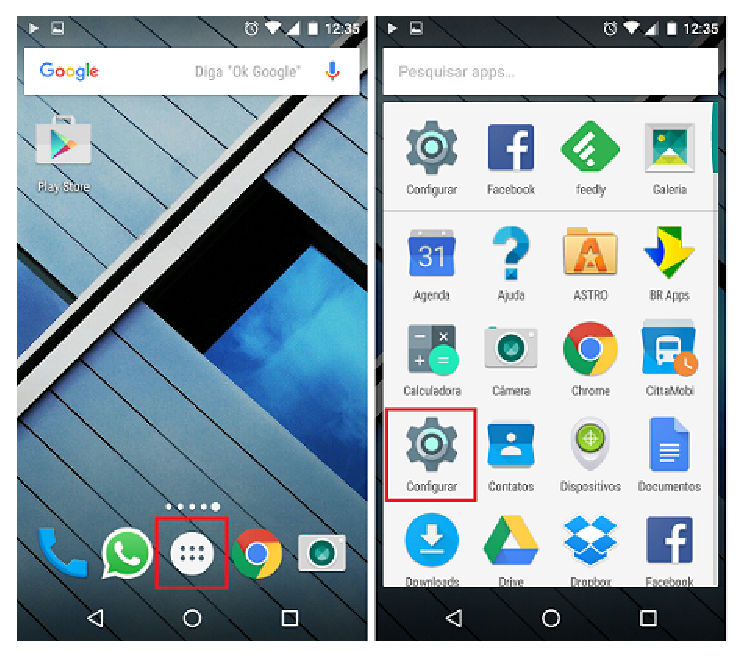
\includegraphics{imagem1.eps}
  \caption{O bot\~ao Aplicativos e o bot\~ao Configurar, ambos destacados em vermelho}
\end{figure}

Como a interface varia conforme os dispositivos Android, devido \`a customiza\c c\~ao do sistema por parte de alguns fabricantes e operadoras de celulares, algumas instru\c c\~oes talvez n\~ao se apliquem diretamente ao dispositivo utilizado pelo leitor. Um exame mais detalhado nas configura\c c\~oes do dispositivo por parte do usu\'ario, deve resolver este problema.   

Tamb\'em \'e necess\'ario enfatizar que estas recomenda\c c\~oes tratam da vers\~ao 6.0 do sistema Android (apelidada de Marshmallow). O leitor pode verificar se esta \'e a vers\~ao presente em seu dispositivo seguindo as instru\c c\~oes logo abaixo.

\begin{enumerate}
\item Pressionar o bot\~ao Aplicativos
\item Pressionar Configurar
\item Deslizar at\'e a se\c c\~ao Sistema
\item Pressionar Sobre o telefone
\item Verificar se Vers\~ao do Android \'e 6.0 ou superior
\end{enumerate}

\begin{figure}[h]
	\centering
	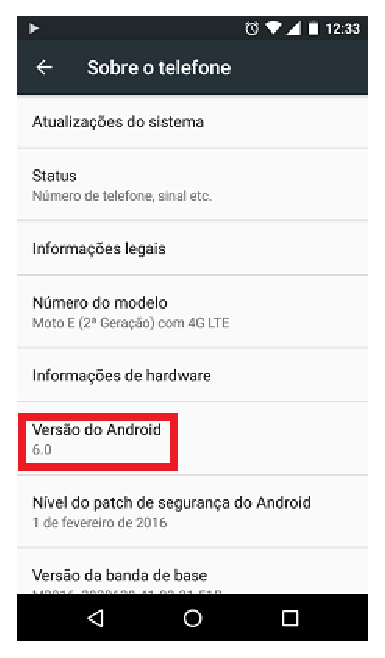
\includegraphics{imagem2.eps}
	\caption{A vers\~ao presente no dispositivo usado para testes, destacada em vermelho}
\end{figure}

Vale lembrar que o autor n\~ao se responsabiliza por eventuais danos causados em dispositivos Android decorrentes da aplica\c c\~ao das configura\c c\~oes recomendadas aqui. Por isso, \'e sugerido que, se poss\'ivel, estas recomenda\c c\~oes sejam aplicadas inicialmente em aparelhos de teste para, apenas depois, serem aplicadas em outros dispositivos. 

Realizar backups das informa\c c\~oes contidas no dispositivo tamb\'em \'e uma pr\'atica recomend\'avel para a recupera\c c\~ao de informa\c c\~oes importantes, caso ocorram eventuais problemas. Seguem logo abaixo instru\c c\~oes para a realiza\c c\~ao de backups em dispositivos Android:

\begin{enumerate}
\item Pressionar o bot\~ao Aplicativos
\item Pressionar Configurar
\item Deslizar at\'e a se\c c\~ao Pessoais
\item Pressionar Fazer backup e redefinir
\item Pressionar Backup dos dados 
\item Ativar o backup dos dados
\item Voltar \`a tela anterior, e ativar a Restaura\c c\~ao autom\'atica
\item Na mesma tela, Em Conta de backup, definir a conta em que o backup ser\'a realizado   
\end{enumerate}

\begin{figure}[h]
	\centering
	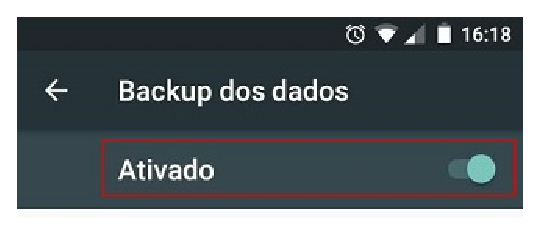
\includegraphics{imagem3.eps}
	\caption{O controle de ativa\c c\~ao do backup, destacado em vermelho}
\end{figure}

